% =========================================================================
% CHAPTER 9 — RESULTS
% =========================================================================

\chapter{Results}
\label{ch:results}

\noindent
{\rmfamily\itshape
\begin{tabular}[t]{@{}l@{\hspace{0.3cm}}p{12.5cm}@{}}
\textls[50]{\textbf{Addressed:}} &
\textls[50]{Descriptive analysis · Coding outcomes · Exploratory comparison}
\end{tabular}
}

\vspace{0.5cm}

This chapter reports what the coded responses show: the sample, the coding outcome for each scene, the frequency of the streamfunction misconception, the relationship between confidence and correctness, and the distribution of the emergent codes across conditions. Their interpretation, and their relation to the expectations of Chapter~\ref{ch:userstudy}, is left to Chapter~\ref{ch:discussion}. Given the sample of twenty-five, all figures are descriptive; the three exploratory tests below are labelled as such and are not treated as inferential.\footnote{All counts and tables in this chapter were recomputed directly from the coded response set. The full result tables are stored in the project results folder.}

% -------------------------------------------------------------------------
\section{Sample Composition}
\label{sec:res-sample}

Twenty-five participants completed the study, twelve in the control condition and thirteen in the experimental condition. Most were aged 25 to 34 (17 of 25). The sample was highly educated: fifteen held a master's degree, nine a bachelor's, and one an upper-secondary qualification (Figure~\ref{fig:demographics}). Fields of study and work were varied --- engineering, the sciences, the humanities, healthcare and the arts --- with no field represented by more than two participants.

Self-rated familiarity was low for the specific system and moderate for the related skills. Familiarity with the AMOC was very low (mean 1.84 on a ten-point scale), familiarity with climate topics moderate (4.88), and familiarity with reading data visualisations the highest of the three (6.20).

A balance check compared the two conditions on these measures (Figure~\ref{fig:balance}). The experimental group was not higher than the control group on any of them, and was slightly lower on all three; the largest difference was in data-visualisation familiarity (5.54 against 6.92), which a Mann--Whitney comparison placed at $p \approx 0.09$, exploratory.\footnote{This check tests whether the groups started from a similar level, not whether the study hypotheses hold. The direction of this difference matters for the Scene~I misconception (\S\ref{sec:res-misconception}) and is returned to in Chapter~\ref{ch:discussion}.}

% -------------------------------------------------------------------------
\section{Structural Comprehension by Scene}
\label{sec:res-structure}

The share of responses coded \emph{grasped} varied sharply across the three scenes, and the direction of the difference between conditions was not the same in each (Figure~\ref{fig:grasped}).

In \textbf{Scene~I} (opposing directions with depth), the two conditions were close. Two-thirds of control responses (66.7\%) and a similar share of experimental responses (69.2\%) were coded grasped. In \textbf{Scene~II} (recurrence), no control participant was coded grasped (0 of 12), against 23.1\% in the experimental condition (3 of 13); partial codes also rose across the same comparison, from two to five. In \textbf{Scene~III} (change in model agreement over time), the pattern was reversed. Every control participant was coded grasped (12 of 12, 100\%), against 76.9\% in the experimental condition (10 of 13).

A Fisher exact test was run once per scene, on the two-by-two table of grasped against not-grasped. It returned $p = 1.00$ for Scene~I, $p = 0.22$ for Scene~II and $p = 0.10$ for Scene~III. All three are exploratory.\footnote{Three tests only, one per scene, fixed in advance. Not-grasped pools \emph{partial} and \emph{not\_grasped}. No test is corrected for multiple comparisons or read as inferential, in keeping with the sample size stated in Chapter~\ref{ch:userstudy}.} Table~\ref{tab:grasped-counts} gives the underlying counts.

\begin{table}[htbp]
\centering
\caption[Structural coding outcomes by condition and scene]{Counts of \emph{grasped}, \emph{partial} and \emph{not grasped} by condition and scene. The percentages in the text are of the condition total (control $n=12$, experimental $n=13$).}
\label{tab:grasped-counts}
\small
\renewcommand{\arraystretch}{1.3}
\begin{tabularx}{\textwidth}{@{}l l *{3}{>{\centering\arraybackslash}X} @{}}
\toprule
\textbf{Scene} & \textbf{Condition} & \textbf{Grasped} & \textbf{Partial} & \textbf{Not grasped} \\
\midrule
I   & Control      & 8 & 3 & 1 \\
I   & Experimental & 9 & 2 & 2 \\
\midrule
II  & Control      & 0 & 2 & 10 \\
II  & Experimental & 3 & 5 & 5 \\
\midrule
III & Control      & 12 & 0 & 0 \\
III & Experimental & 10 & 3 & 0 \\
\bottomrule
\end{tabularx}
\end{table}

% -------------------------------------------------------------------------
\section{The Streamfunction Misconception}
\label{sec:res-misconception}

A diagnostic code, S1-MISC-INT, recorded whether a participant read the height of the streamfunction curve as the speed of the water at that depth, rather than as the cumulative transport. It was present in 14 of the 25 Scene~I responses.

Its frequency differed by condition: 33.3\% of control responses against 76.9\% of experimental ones. Split instead by self-rated data-visualisation familiarity, it was present in 76.9\% of participants at or below the sample midpoint and in 33.3\% of those above it (Figure~\ref{fig:misconception}).

The code was independent of whether the scene was grasped: several participants who correctly described the opposing directions still read the curve's height as speed, carrying both the grasped verdict and the misconception.\footnote{Because the experimental condition also had lower mean data-visualisation familiarity (\S\ref{sec:res-sample}), condition and familiarity are partly confounded at this sample size. The two panels of Figure~\ref{fig:misconception} are therefore not independent, and their joint reading is exploratory. This point is taken up in Chapter~\ref{ch:discussion}.} Three participants explicitly distinguished cumulative transport from velocity and did not carry the code; two of them also asked, unprompted, that the axis be labelled to show which quantity it represented.

% -------------------------------------------------------------------------
\section{Confidence and Correctness}
\label{sec:res-confidence}

Mean confidence was higher for grasped responses than for non-grasped ones in every scene, but the size of the gap varied (Figure~\ref{fig:confidence}). It was widest in Scene~II (6.33 against 4.27) and Scene~III (6.32 against 4.67). It was narrowest in Scene~I, where non-grasped responses still averaged 6.0 against 6.82 for grasped ones.

The pre-registered definition of a confidently-wrong response was a confidence of at least seven together with a \emph{not\_grasped} verdict. Under this definition, no such case appeared in Scene~I. A wider reading, which also admits \emph{partial} verdicts, identified four Scene~I participants (P02, P04, P12 and P17) who rated their confidence at seven or above while coding only partial. Each of these four carried the streamfunction misconception.\footnote{This wider reading is reported as a post-hoc observation and is kept separate from the pre-registered definition, which returns no cases in Scene~I. The four participants are marked in Figure~\ref{fig:confidence}.} Two further cases appear in Scene~II under the same wider reading, one in each condition, and none in Scene~III.

% -------------------------------------------------------------------------
\section{Emergent Codes}
\label{sec:res-emergent}

The coding also surfaced patterns not part of the pre-specified grid. These are reported as post-hoc and kept separate from the structural targets.\footnote{The full list of emergent codes, including those occurring only once, is given in Appendix~\ref{app:protocols}; Figure~\ref{fig:emergent-full} shows all of them by condition. Only the three recurring codes are described here.} Three occurred often enough to report by condition (Figure~\ref{fig:emergent}). \textsc{Interaction-aided}, marking a response that attributed its understanding to acting on the display (pausing, rewinding, isolating), appeared 12 times, all in the experimental condition. \textsc{Static-limit-named}, marking a response that named the absence of a temporal ordering as the reason it could not tell whether the system revisited earlier states, appeared 4 times, all in the control condition. \textsc{Anomaly-confusion}, marking difficulty with the usual/unusual encoding, appeared 6 times, once in the control condition and five times in the experimental.

% -------------------------------------------------------------------------
% FIGURES
% -------------------------------------------------------------------------

\begin{figure}[htbp]
\centering
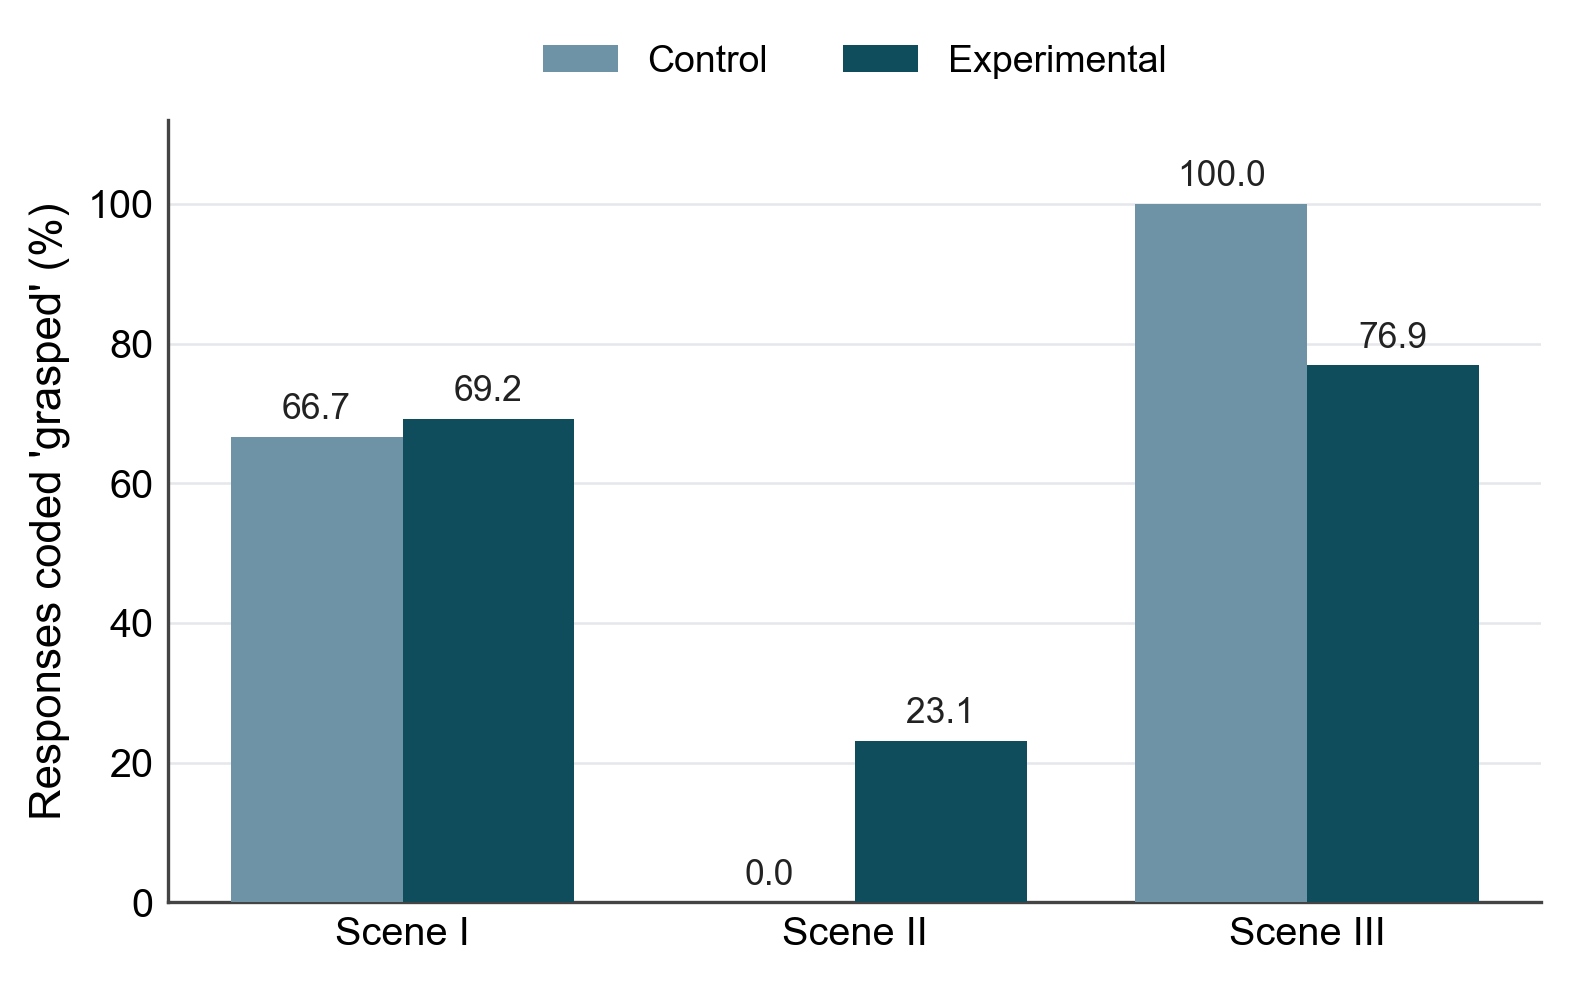
\includegraphics[width=\textwidth]{figures/results/F1_grasped_by_condition_scene.png}
\caption[Structural comprehension by condition and scene]{Percentage of responses coded \emph{grasped} by condition, for each scene. The direction of the difference between the two conditions is not the same across the three scenes.}
\label{fig:grasped}
\end{figure}

\begin{figure}[htbp]
\centering
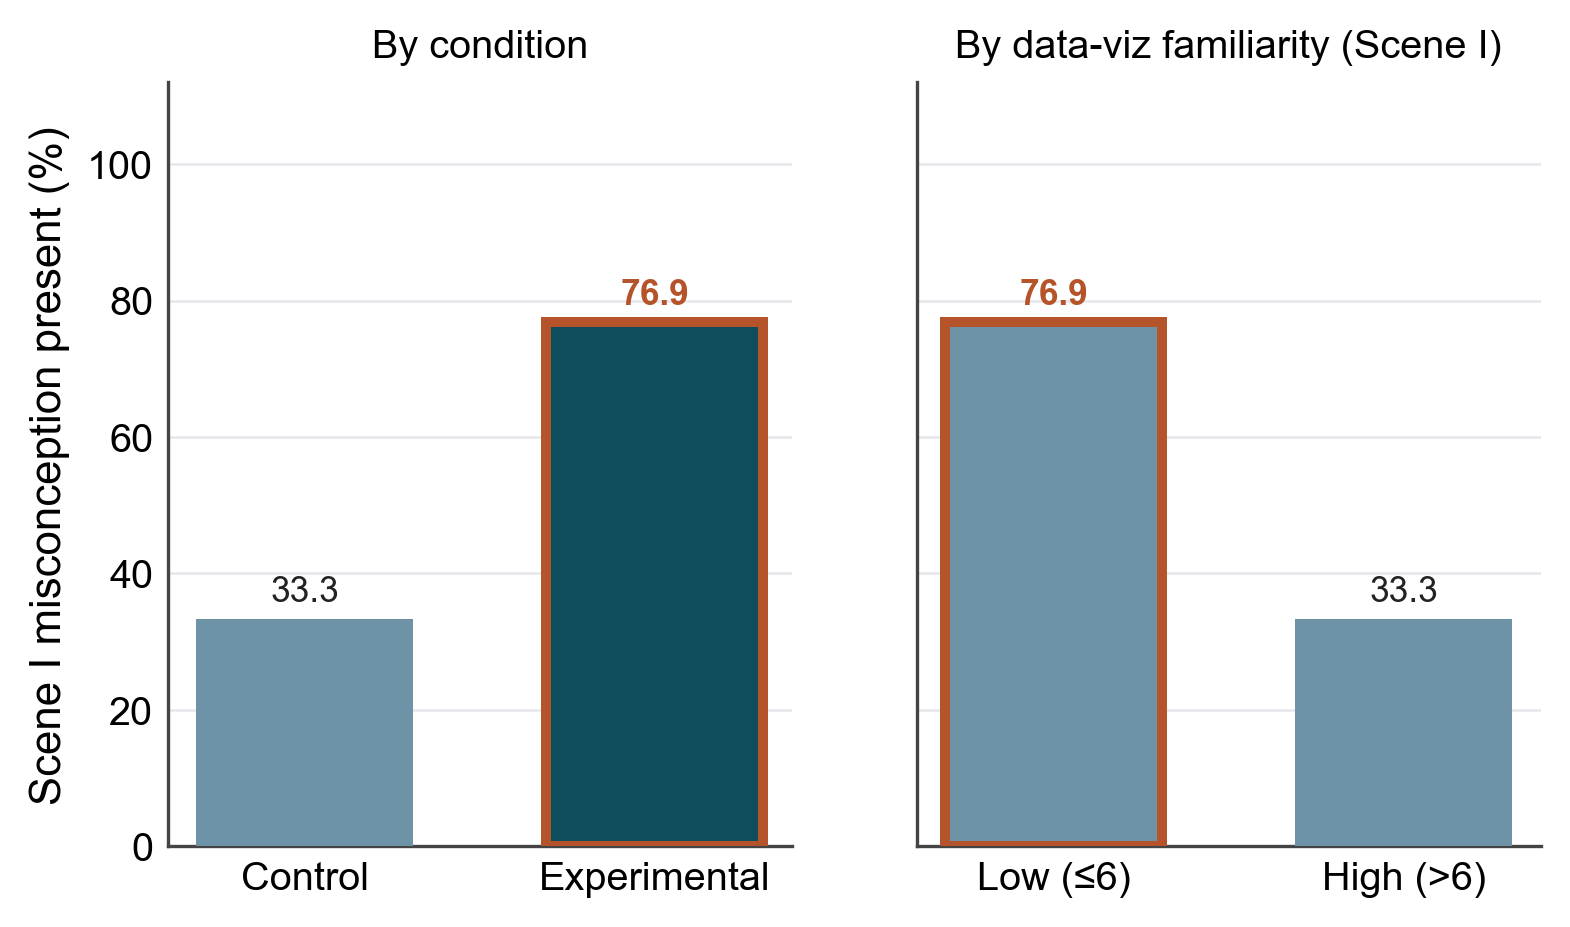
\includegraphics[width=\textwidth]{figures/results/F2_misconception.png}
\caption[The streamfunction misconception, by condition and by familiarity]{Presence of the S1-MISC-INT misconception in Scene~I. Left: by condition. Right: by self-rated data-visualisation familiarity. The two panels are partly confounded (see \S\ref{sec:res-misconception}).}
\label{fig:misconception}
\end{figure}

\begin{figure}[htbp]
\centering
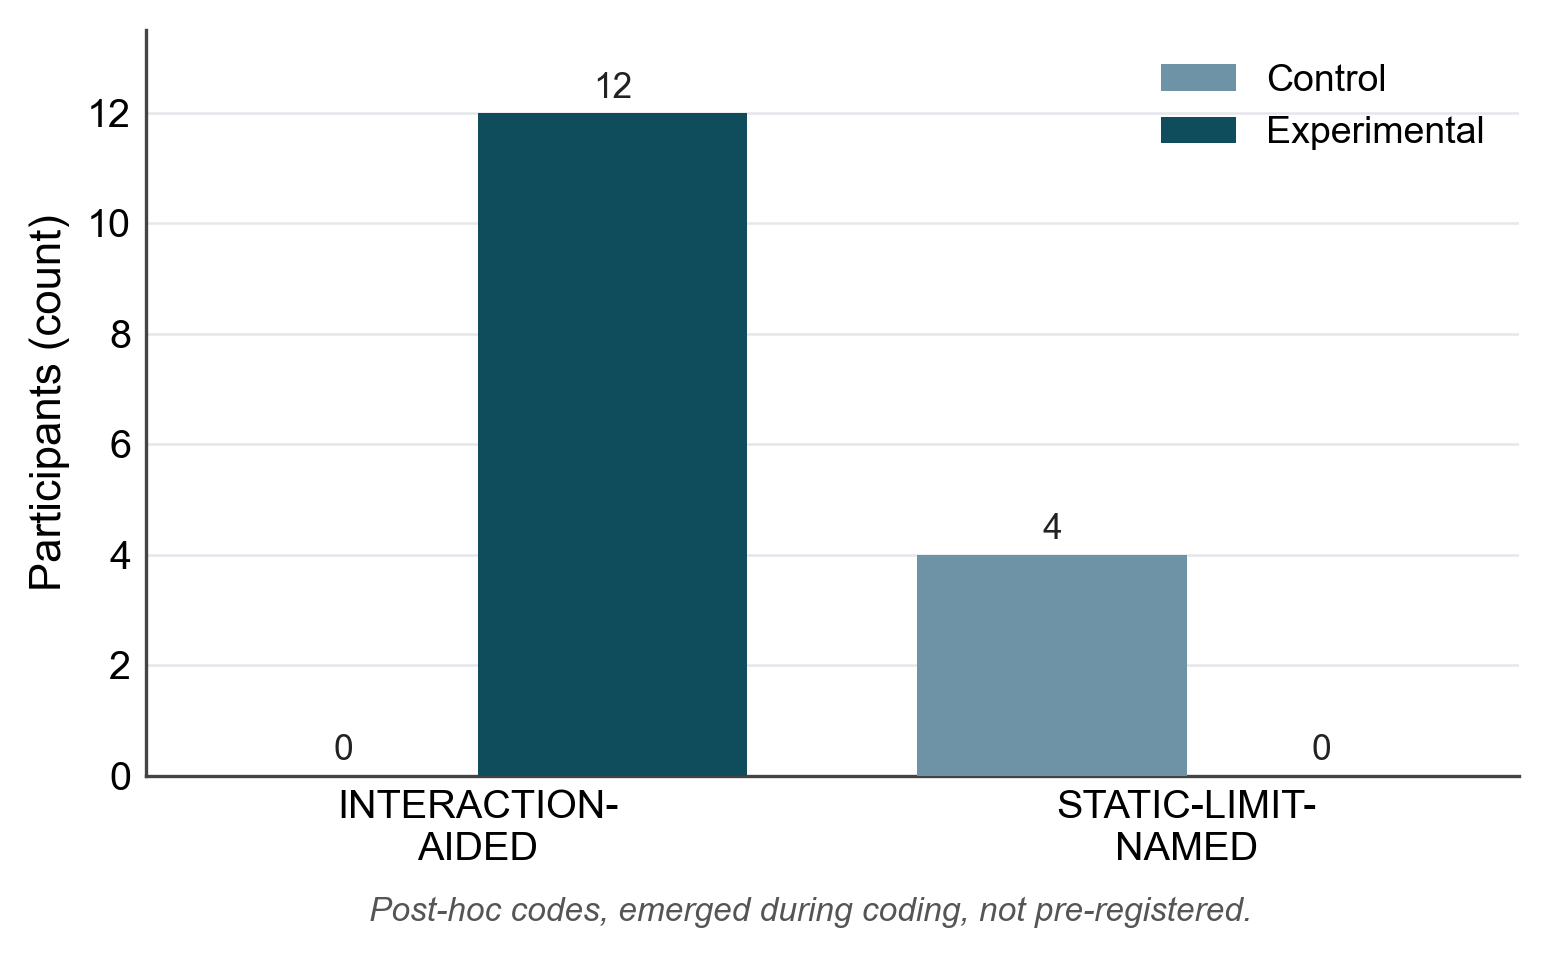
\includegraphics[width=\textwidth]{figures/results/F3_emergent_mechanism.png}
\caption[Recurring emergent codes by condition]{The two mirror-image emergent codes by condition. Post-hoc codes, emerged during coding, not pre-registered.}
\label{fig:emergent}
\end{figure}

\begin{figure}[htbp]
\centering
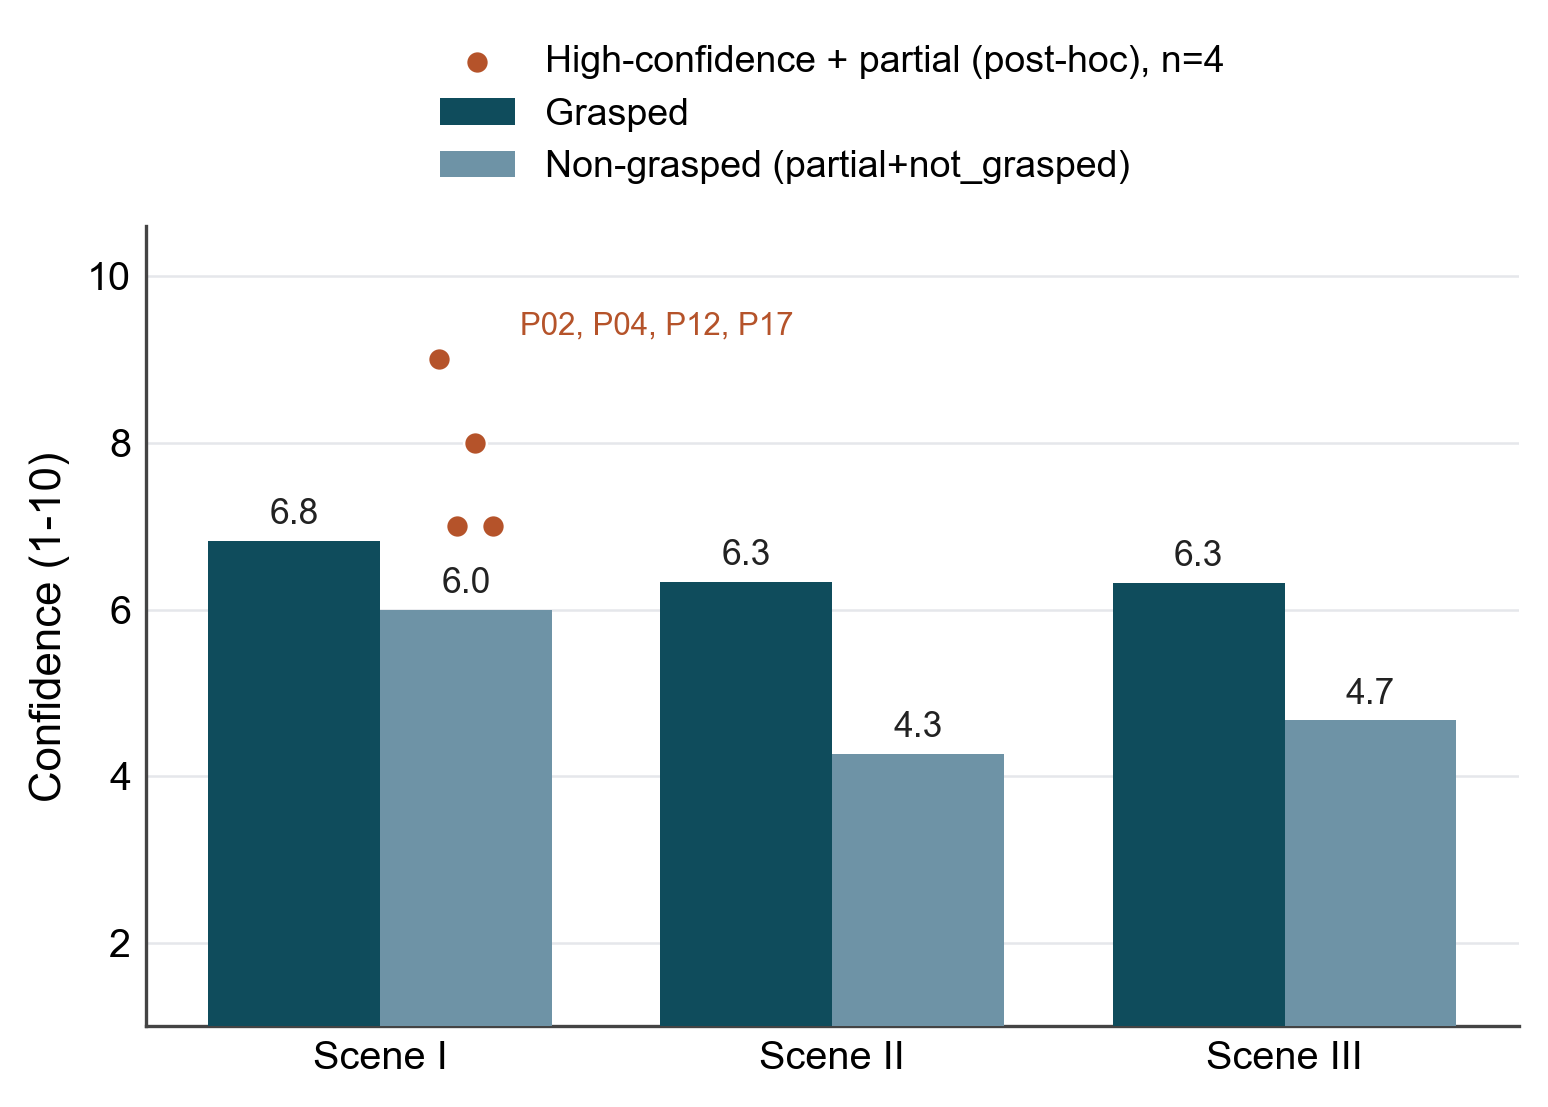
\includegraphics[width=\textwidth]{figures/results/F4_confidence_by_correctness.png}
\caption[Confidence by correctness and scene]{Mean confidence of grasped against non-grasped (partial and not-grasped pooled) responses, by scene. The four highlighted points mark Scene~I participants with confidence $\geq 7$ and a partial verdict (post-hoc reading; see \S\ref{sec:res-confidence}).}
\label{fig:confidence}
\end{figure}

\begin{figure}[htbp]
\centering
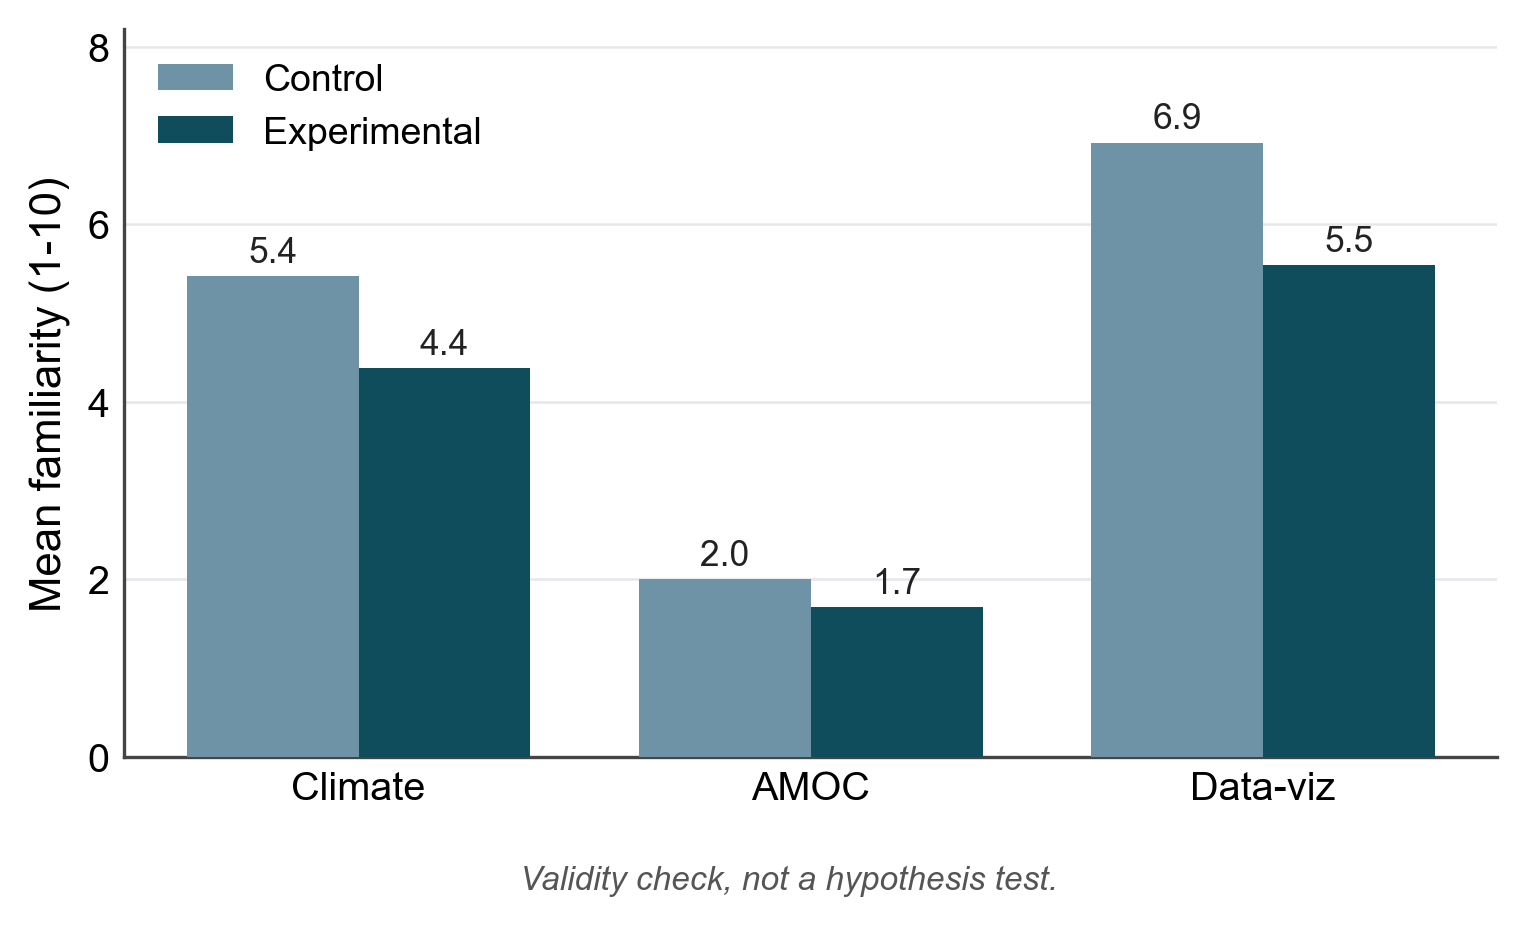
\includegraphics[width=\textwidth]{figures/results/S1_balance_familiarity.png}
\caption[Balance check: familiarity by condition]{Mean self-rated familiarity on the three measures, by condition. A check of group equivalence, not a hypothesis test.}
\label{fig:balance}
\end{figure}

\begin{figure}[htbp]
\centering
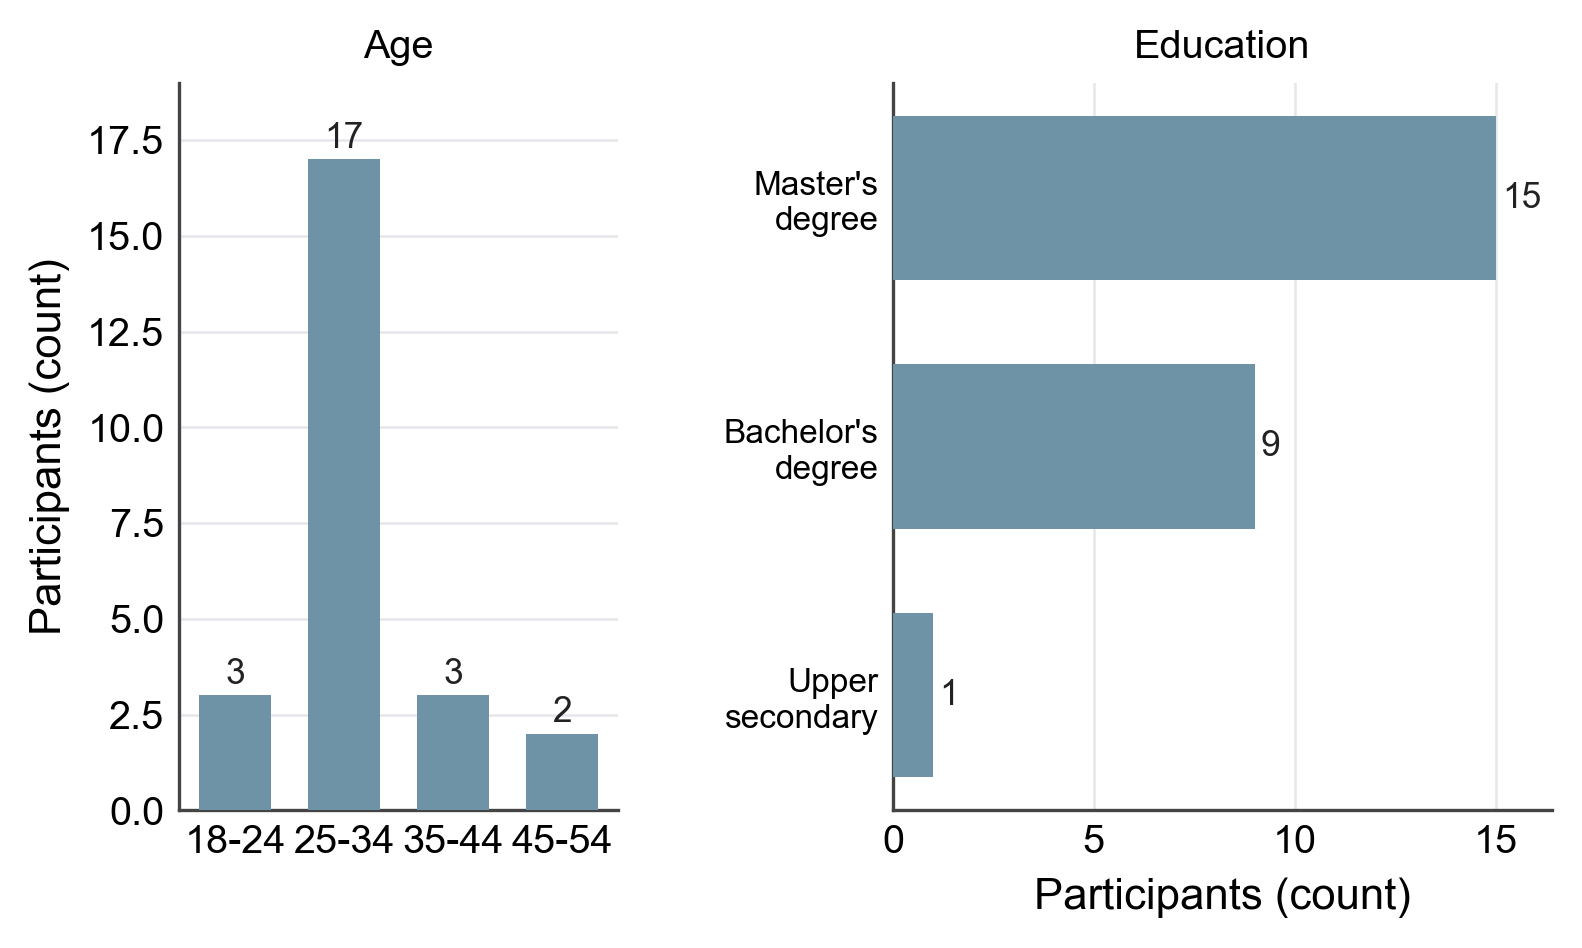
\includegraphics[width=\textwidth]{figures/results/S2_demographics.png}
\caption[Sample demographics]{Distribution of age band and highest level of education across the sample.}
\label{fig:demographics}
\end{figure}

\begin{figure}[htbp]
\centering
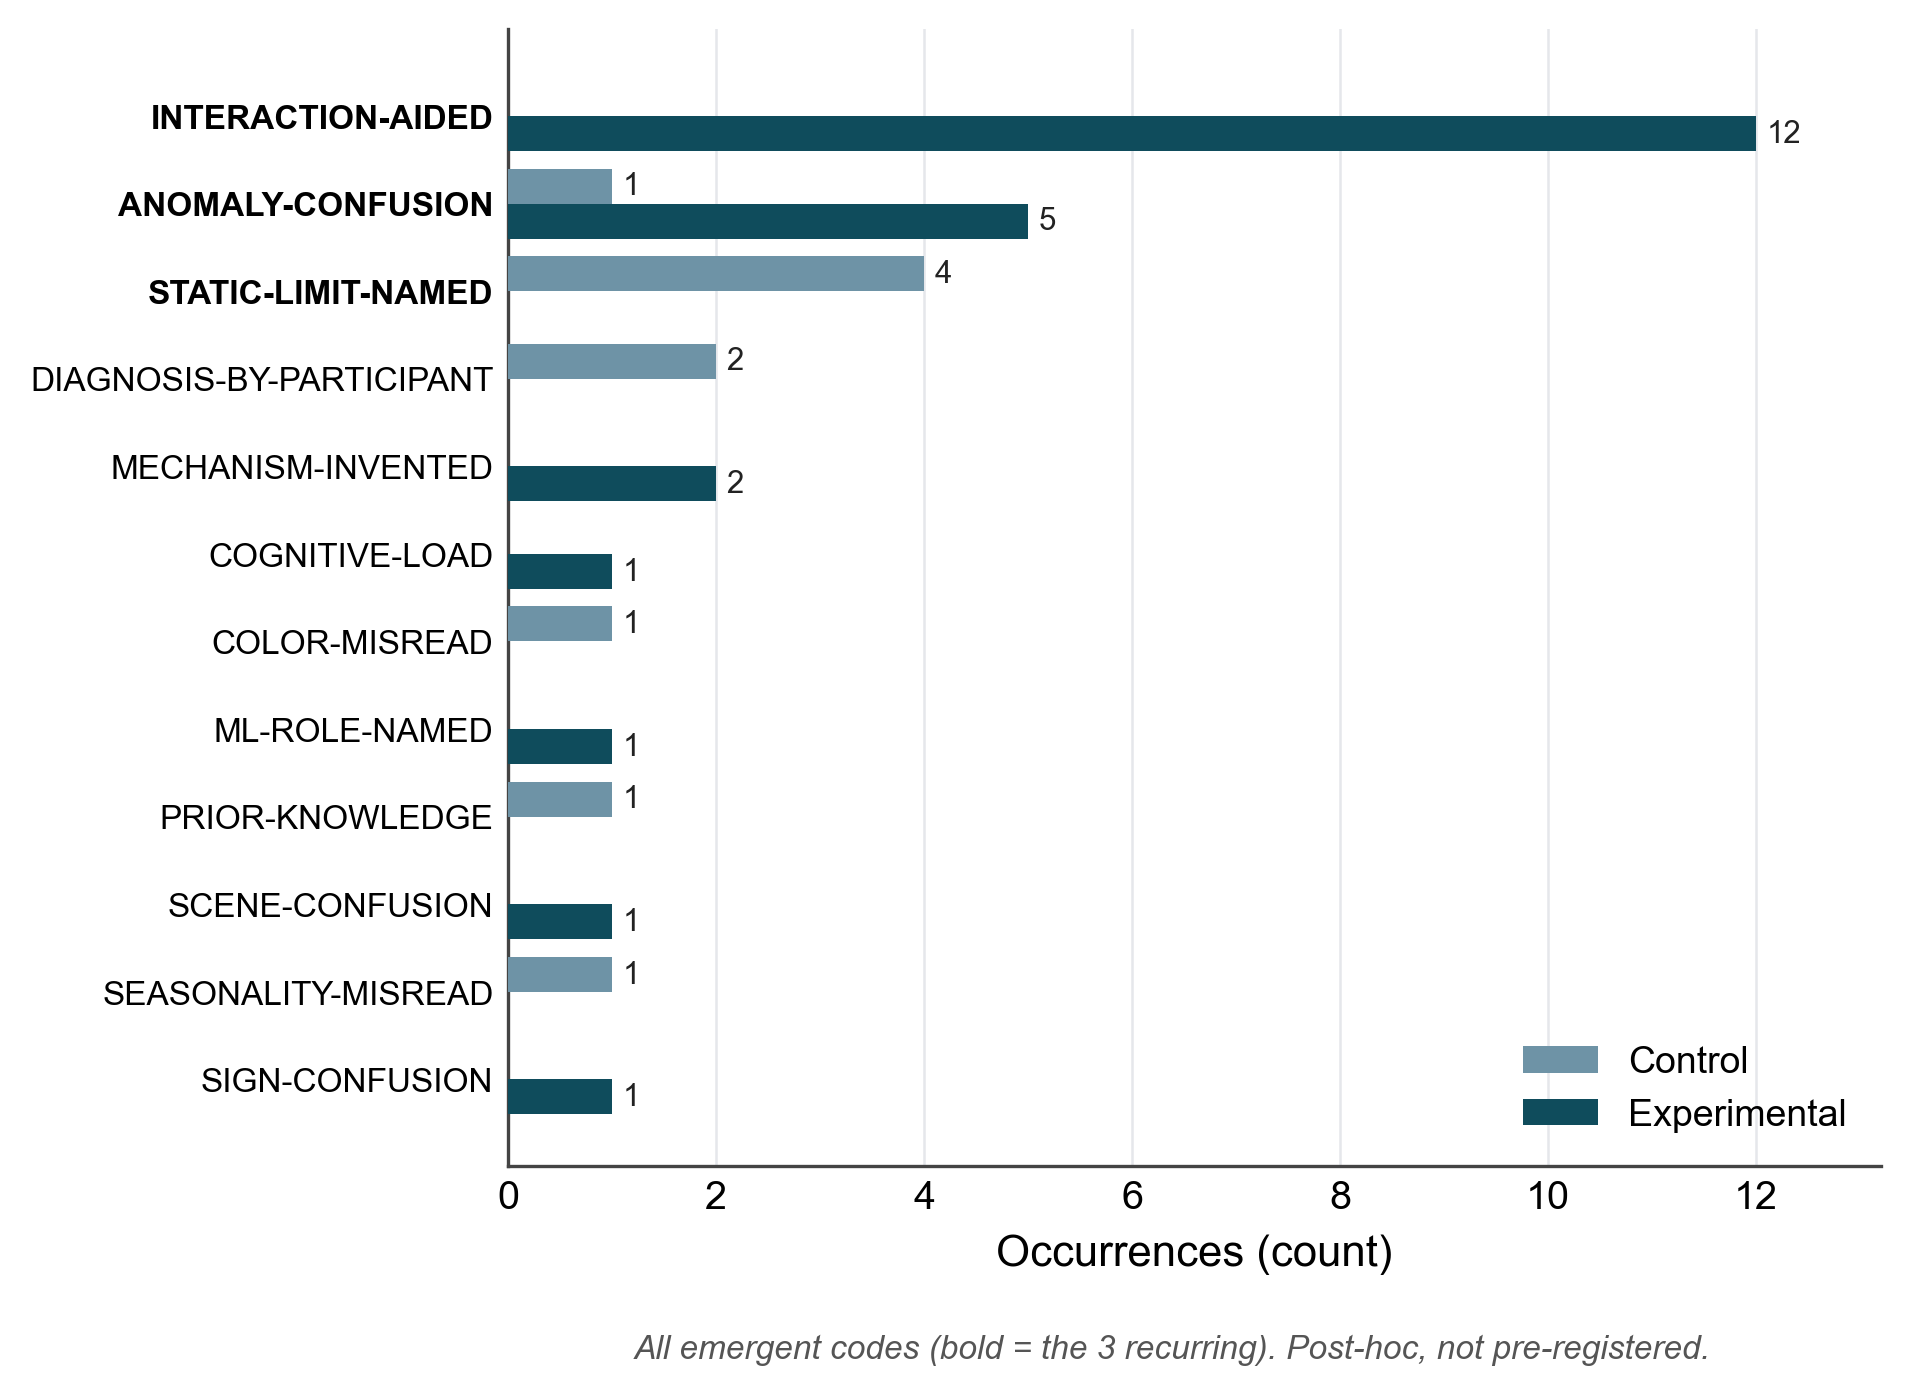
\includegraphics[width=\textwidth]{figures/results/S4_emergent_all_codes.png}
\caption[All emergent codes by condition]{The complete list of emergent codes by condition. Bold marks the three recurring codes. All are post-hoc and not pre-registered.}
\label{fig:emergent-full}
\end{figure}